\chapter{}{Multi-Model Approach to Solar Irradiance Forecasting}

\subchapter{Overview}
A variety of solar irradiance forecasting techniques targeted at different forecast horizons have been developed using different input data based on the temporal variability of the forecast horizon, and the spatial scale of the input data. As shown in Fig.~\ref{fig:fig_variability}, intra-hour forecasts can follow from statistical time-series based models on surface measurements, or from tracking the cloud-motion observed with ground-based, all-sky cameras \cite{multimodal_intrahour}. Input data from satellite imagery tracking cloud motion has been shown to be useful for a forecast horizon between 30 minutes and 6 hours. For days-ahead forecast horizon, regional and global numerical weather prediction models, predicting the evolution of the atmospheric system have been shown to be more appropriate and accurate.

\begin{figure}[htbp]
    \begin{center}
    	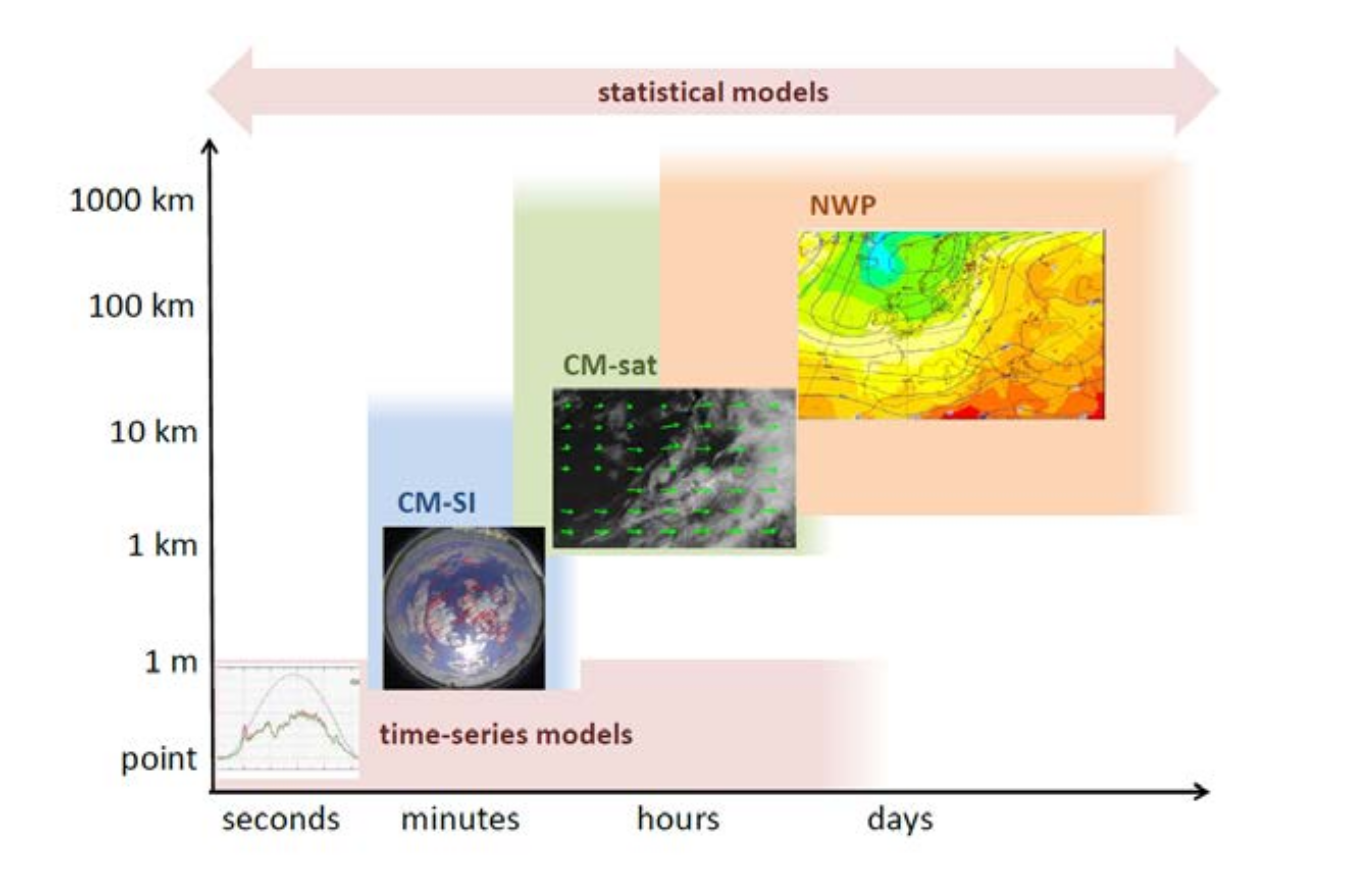
\includegraphics[width=0.75\textwidth]{chapter3/fig_variability.png}
    	\label{fig:fig_variability}
    	\caption[Solar forecasting methods based on varied spatial and temporal scales]{Solar forecasting methods based on varied spatial and temporal scales\cite{multimodel_figure1}.}
    \end{center}
\end{figure}

\par The numerical weather prediction models derive their initial conditions from different ground and airborne sensors from across the world, and based on equations describing the physical processes occurring in the atmosphere, forecast a parameter into the forecast horizon. The National Oceanic and Atmospheric Administration (NOAA) operates a variety of numerical weather prediction models with their spatial resolution ranging from approximately 10 km - 50 km, and their temporal reoslution typically being 1 hour or 3 hours, and which are normally updated every 6 hours \cite{multimodel_bestpractices}. 

\par In this work, we intended to forecast solar irradiance captured at the solar farm in Athens, Georgia for a forecast horizon of 24 hours. For this purpose, a mesoscale model which can predict parameters describing cloudiness such as \textit{North American Mesoscale (NAM)} Forecast System \cite{multimodel_nam} was used. Typical weather variables known to affect solar irradiance forecasting systems such as air temperature, geopotential height, cloud cover, visibility, wind speed, dew point temperature, air pressure, downwelling shortwave radiation flux, downwelling longwave radiation flux, and humidity were evaluated so as to gauge their effect on the solar irradiance predictions. This enabled a cut in computational cost of modeling and also led to an improvement in the performance of the model.

\par Downwelling shortwave radiation flux, synonymous with global horizontal irradiance (GHI) is measured by NWP models using columnar radiative transfer models (RTM). However, the direct output from the mesoscale models has shown severe deviations between forecasted and real irradiance \cite{multimodel_ghi}. While the usage of additional weather variables in machine learning models have shown to improve the post-processing of NWP models with site-specific information, one fact which has to be taken into consideration is that there is a significant variability in the GHI measured by the NWP models depending on the cloud conditions. As a matter of fact, Mathiesan et al \cite{multimodel_overpredict} found that the NAM forecast model tends to overpredict GHI in clear sky conditions by up to 40 percent.

\par There are multiple formulations which have been extensively discussed in literature which compute the irradiance metrics from environmental conditions such as cloud cover, and can be broadly classified into decomposition models and isotropic models. Using assumptions on solar geometry and transmittance, the former are used to estimate direct beam and diffuse irradiance. The latter are useful for approximating daily solar radiation reaching tilted surfaces. The irradiance metrics retrieved using either of these models can be used to empirically estimate global horizontal irradiance, which can further be used to correct the bias in GHI forecasts recorded by the NWP models. Such a bias correction can lead to an improvement in the post-processing of the input data for the machine learning models with respect to the solar irradiance observations from the solar farm.

\subsubchapter{Numerical Weather Prediction (NWP) Models}
Meteorological forecasts from Numerical Weather Prediction (NWP) models have successfully been employed for the purpose of solar forecasting. The making of a weather forecast revolves around assessing the current weather situation, assimilating observational information, and projecting this initial state into future based on the laws of thermodynamics. One of the major challenges faced in this process is determining the range of area to observe. As shown in Fig.~\ref{fig:fig_variability}, the further the forecasting of the weather conditions, i.e, higher the forecast horizon, the wider is the range of area that needs to be observed. 

\par Multiple weather prediction models, both global and regional, depending on the spatial domain, are maintained by the National Oceanic and Atmospheric Administration (NOAA). Global Forecast System (GFS) is one of the widely-known global weather prediction models, while North America Mesoscale (NAM), Rapid Refresh (RAP), High Resolution Rapid Refresh (HRRR) are popular regional weather prediction models in the United States. For our experiments, we chose the North America Mesoscale (NAM) model data and created a weather forecast dataset spanning the years 2017 and 2018, though a few forecasts are missing sporadically.

\begin{figure}[htbp]
    \begin{center}
    	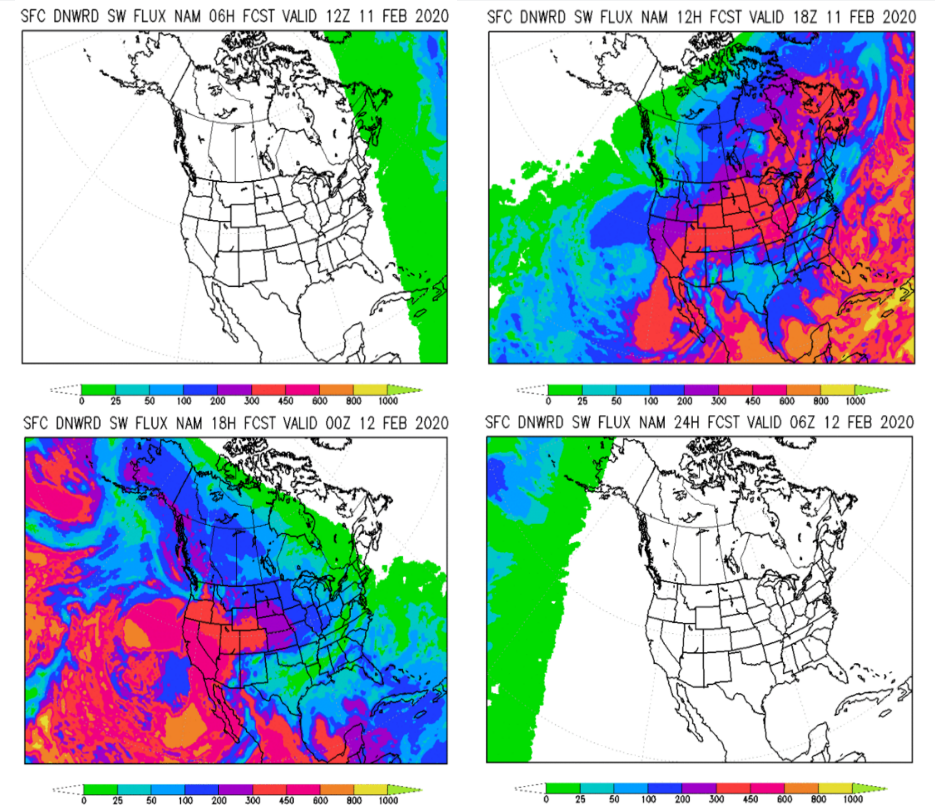
\includegraphics[width=0.85\textwidth]{chapter3/fig_nam_dswrf.png}
    	\label{fig:fig_nam_dswrf}
    	\caption[Downward shortwave radiation flux parameter for 06h, 12h, 18h, 24h forecasts in a day for NAM model data]{Downward Shortwave Radiation Flux parameter from NAM data over North America domain for 06h forecast (top-left), 12h forecast (top-right), 18h forecast (bottom-left) and 24h forecast (bottom-right) for 11th February, 2020.}
    \end{center}
\end{figure}

\par The North America Mesoscale (NAM) Forecast System provides high resolution forecasts over North America for a forecast horizon of 84 hours, the first 36 of which are at a one hour temporal resolution, and the remaining thereafter, at a 3 hour temporal resolution. The forecasts are published for a grid spanning approximately $12km$ x $12 km$ across the continental United States, which are released four times daily at 00h, 06h, 12h and 18h. Following the update in 2017, the current version of the NAM model follows Betts-Miller convection for parameterization of physical processes, RTM-based longwave and shortwave prediction scheme, and an updated Ferrier-Aligo predictive cloud scheme \cite{multimodel_cloud}.

\par Dozens of parameters are available in a NAM model data grid pertaining to environmental components such as altitude, atmospheric pressure, atmospheric radiation, air temperature, water vapour, atmospheric winds, precipitation, soil properties and cloud cover. The features are spread across 60 vertical levels in a 0 - 3 km layer, and across 39 pressure levels from 50mb to 1000mb at 25mb intervals. Among these parameters, in Fig. ~\ref{fig:fig_nam_dswrf}\footnote{NAM forecast snapshots retrieved from: \url{https://www.emc.ncep.noaa.gov/mmb/mmbpll/etapll}}, the averaged downwelling short-wave radiation flux over North America is reported.

\subsubchapter{PVLIB Forecast Modeling}
Holmgrem et al \cite{pvlib_Holmgren2018} contributed to building pvlib-python\footnote{https://github.com/pvlib/pvlib-python} an open source, python-based tool, ported from the PVLIB MATLAB toolbox developed at the Sandia National Laboratories. This software provides a set of functions and classes for simulating the performance of the photovoltaic energy systems, with implementations of algorithms related to solar energy. In particular, the 'forecast' module contains objects to obtain weather forecast data from NOAA/NCEP/NWS models including the GFS, NAM, RAP, HRRR, and the NDFD, retrieved from the UNIDATA THREDDS servers, and convert that data into a PV power forecast. 

\par For our experiments, we created a NAM weather forecast dataset for the years of 2017 and 2018, retrieved from the NCEP servers. Meanwhile, pvlib-python retrieves NAM CONUS 12km resolution forecasts from THREDDS servers. The key difference between each of the datasets is that the former is a full complement of both the pressure level fields and surface-based fields, while the latter is a full complement of just the surface-based fields. In the forecast module, pvlib-python returns a dataset consisting of the following features: air temperature, wind speed, total clouds, low clouds, mid clouds, high clouds. 

\par To be able to use the pvlib-python functionalities, both the datasets were connected by mapping corresponding surface-level features. pvlib-python helps process the NAM data so as to compute irradiance metrics such as global horizontal irradiance (GHI), diffused horizontal irradiance (DHI) and direct normal irradiance (DNI) from the total cloud cover, using two techniques: Clearsky Scaling, Liu Jordan.


\subsubsection*{Clearsky Scaling}
Global horizontal irradiance can be measured with the help of a pyranometer on a horizontal surface, and thus, is typically, the most common type of irradiance measurement. Knowledge of the clear sky conditions, i.e. absence of clouds, is a key requirement for forecasting all the three irradiance metrics. Several parametric models have been proposed to compute these irradiance metrics from environmental conditions such as atmospheric turbidity, fractional sunshine, perceptible water vapor, etc. Ineichen et al \cite{pvlib_ineichen} formulated a model to compute Linke turbidity independent of the airmass, and global horizontal irradiance under clear sky conditions. Going by Larson et al's \cite{pvlib_larson} work, pvlib-python scales global horizontal irradiance on the basis of the total cloud cover. Furthermore, cloudy sky direct normal irradiance is determined based on the DISC \cite{pvlib_disc} model, and diffused horizontal irradiance is empirically formulated from global horizontal irradiance and direct normal irradiance thus calculated.

\subsubsection*{Liu-Jordan Method}
Decomposition models typically utilize only data pertaining to global radiation to estimate diffuse radiation from global solar irradiation data. They are based on the atmospheric effects in an isolated place, varying according to time of the year, season and climatic conditions \cite{pvlib_liujordan}. Liu et al proposed one of the earliest and simplest models of radiation, the Liu-Jordan model \cite{pvlib_liujordan2}, which presumes that diffuse radiation intensity is distributed uniformly over the whole sky, and helps estimate diffuse radiation on horizontal surfaces. It is also one of the more accurate among isotropic models for estimating diffused radiation on inclined surfaces \cite{pvlib_liujordan3}. This model helps determine direct normal irradiance, global horizontal irradiance from properties such as extraterrestrial flux, transmittance, and optical air mass number; and diffused horizontal irradiance from an empirical equation for diffuse radiation.

\subchapter{Data Collection and Pre-processing}
\subsubsection*{Weather Forecasts}
\par As mentioned in 3.1.1, North America Mesoscale (NAM) model data was collected from the years 2017 and 2018 for experiments. From the NAM model data, surface-level parameters as described in Table \ref{Tab:table_nam_variables} were retrieved and analyzed. NAM model projects each of the features 36 hours into the future at a 1-hour temporal resolution, and subsequent 48 hours at a 3-hour temporal resolution. In this work, we analyze the first 24 hours projections of the features against the corresponding target pyranometer readings.
\begin{table}[h]
\begin{center}
    \label{Tab:table_nam_variables}
    \caption{NWP-NAM variables retrieved for solar forecasting}
    \begin{tabular}{ c c }
    	\toprule
    	Label & Description \\
    	\midrule
    	PRES\_SFC & Air Pressure \\
    	HGT\_SFC & Geopotential Height \\
    	HGT\_TOA & Height at Planetary Boundary Layer \\
    	TMP\_SFC & Air Temperature \\
    	VIS\_SFC & Visibility \\
    	UGRD\_TOA & U-Component of Wind Speed \\
    	VGRD\_TOA & V-Component of Wind Speed \\
    	DSWRF\_SFC & Downward Short-Wave Radiation Flux \\
    	DLWRF\_SFC & Downward Long-Wave Radiation Flux \\
    	TCC\_EATM & Total Cloud Cover (\%) \\
    	\bottomrule
    \end{tabular}
\end{center}
\end{table}

\subsubsection*{Temporal Features}
\par In \cite{Zach_Thesis}, Jones et al. extracted temporal features by taking the sine and cosine of the reference time with periods of one-day and one-year. This was achieved by scaling the epoch representing the reference time by $8.64e+13$ and $3.1536e+16$ respectively. Though the addition of such temporal features results in a considerable improvement in performance, it fails to capture the cyclicity of the reference time in a particular day, or that of the months in a particular year. So, the time of day and time of year were modified to represent the hour in a day and the month in a year respectively, of which the sine and cosine values were added as the temporal features. Furthermore, such temporal features of the reference times representing the day-ahead target variables were also included. 

\subsubsection*{Irradiance Observations}
\par Georgia Power, in collaboration with the University of Georgia set up a 1MW solar facility in Athens, Georgia. The irradiance observations are obtained from three solar arrays in the solar farm, namely array A, array B and array E, representing a dual-axis tracking array, fixed axis array with 200$^{\circ}$(SW) azimuth, and a single-axis tracking array respectively. Each of the solar arrays are installed with thermopile pyranometers from different manufacturers such as Kipp \& Zonen\footnote{\url{https://www.kippzonen.com/}}, and LICOR\footnote{\url{https://www.licor.com/}}.

\begin{figure}[htbp]
    \begin{center}
    	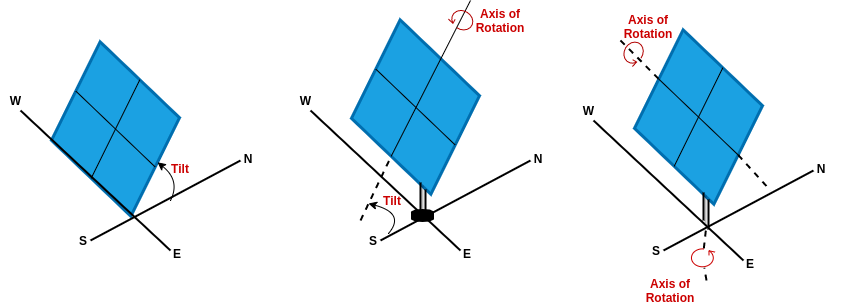
\includegraphics[width=0.85\textwidth]{chapter3/fig_pyranometers.png}
    	\label{fig:fig_pyranometers}
    	\caption[Fixed axis, Single-axis tracking, Dual-axis tracking Solar Arrays]{Fixed axis (left), Single-axis tracking (center), Dual-axis tracking (right) Solar Arrays.}
    \end{center}
\end{figure}


\subsubsection*{Feature Selection}
On the weather forecast features from the NAM dataset as described in 3.2, feature selection was performed using the mutual information metric, and the random forests technique. Mutual information is the measure between two possibly multi-dimensional variables, which quantifies the amount of information obtained from one variable about the other. The relationship detected between the variables can involve either mean, variance or even the higher moments \cite{feature_selection_mi}. For the estimation of mutual information, a non-parametric method based on the entropy estimation from the k-nearest neighbors as described in \cite{feature_selection_mi} and \cite{feature_selection_mi2} was utilized. 

\begin{figure}[htbp]
    \begin{center}
    	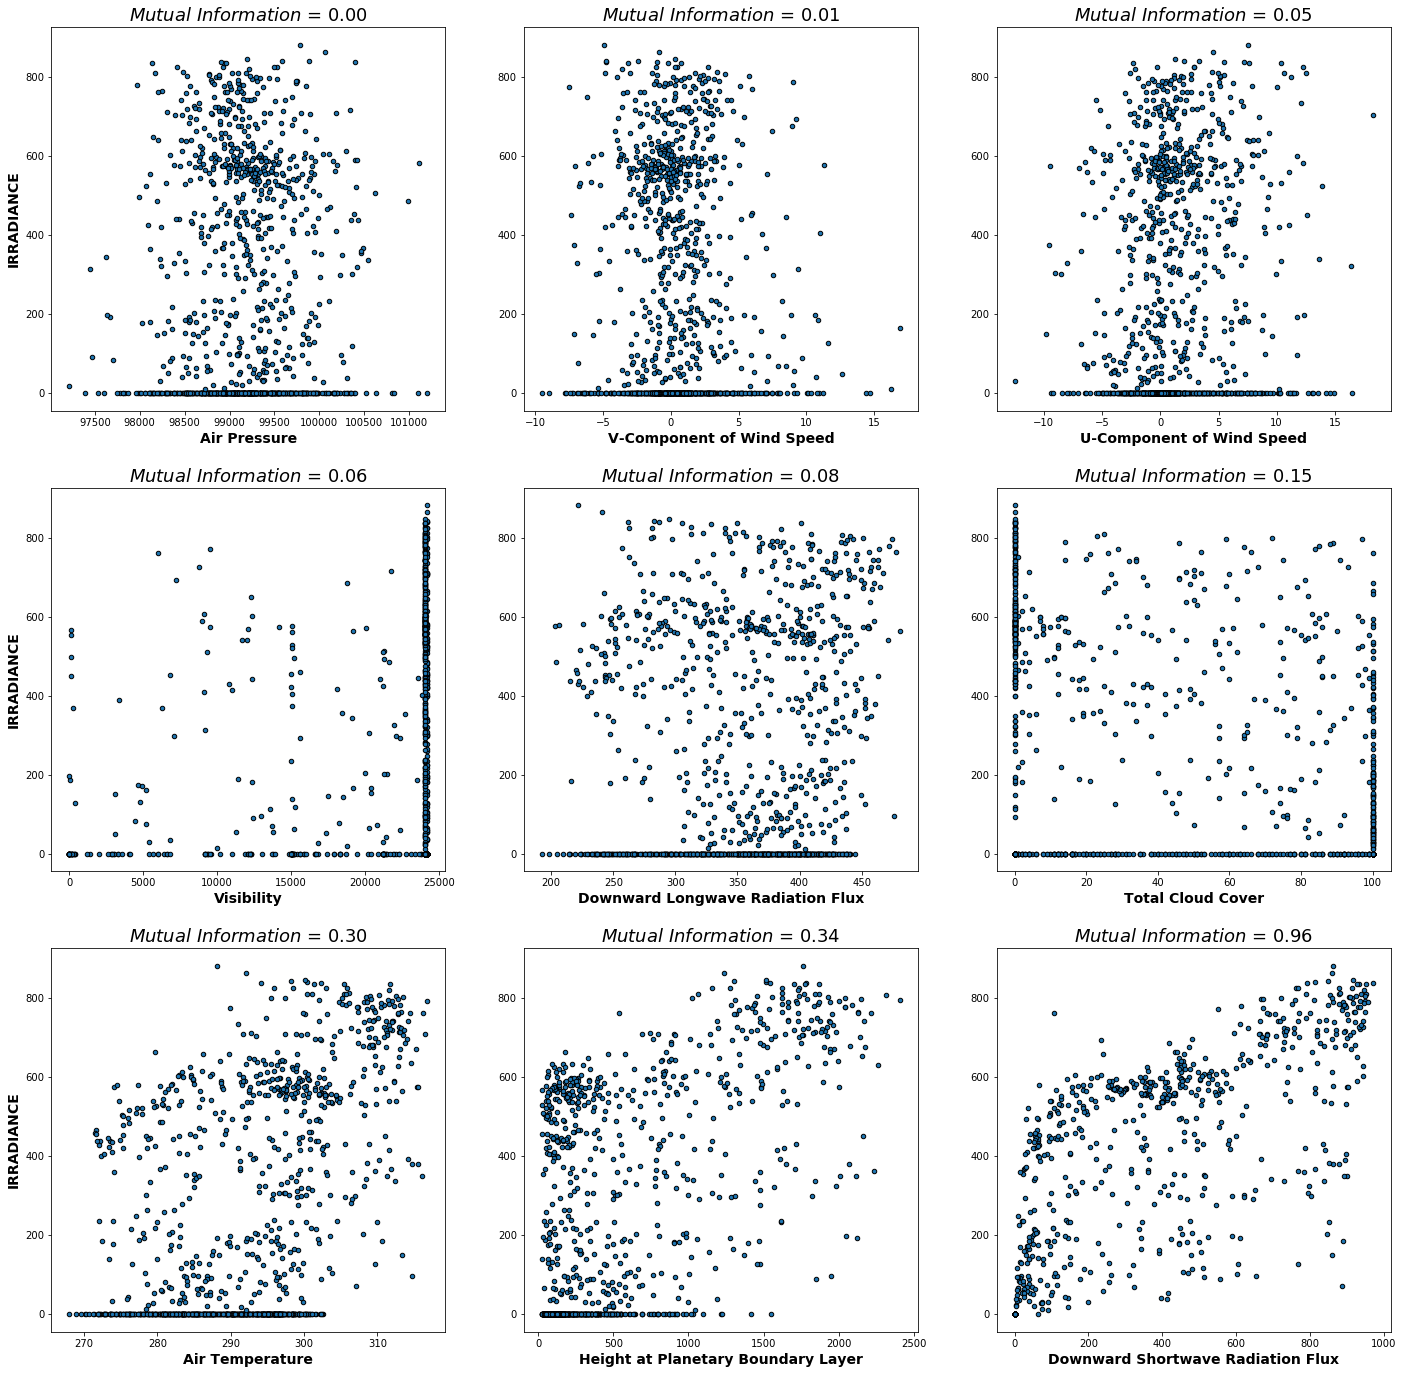
\includegraphics[width=\textwidth]{chapter3/fig_mi_ugabpoa1irr.png}
    	\label{fig:fig_mi_forecast_target_hr1}
    	\caption[Mutual information between NAM feature projection forecast and corresponding solar array B irradiance]{Mutual information between NAM feature projection forecast and corresponding solar array B irradiance.}
    \end{center}
\end{figure}

In Fig.\ref{fig:fig_mi_forecast_target_hr1}, mutual information between NAM feature projection forecast for the first forecast hour in the forecast horizon, and corresponding irradiance observations from array B is shown. It can be observed that downward shortwave radiation flux (DSWRF\_SFC), air temperature (TMP\_SFC), height at planetary boundary layer (HGT\_TOA) and total cloud cover (TCC\_EATM) have a mutual information score greater than 0.1, indicating a higher dependency with the irradiance observations. 

\par Random forests are commonly used for the purpose of feature selection. They are an ensemble learning technique constructed over a variety of randomized decision trees, each of which is built over a random extraction of features and data observations. The training of these randomized decision trees is done so that the Gini Impurity is decreased, and those features are selected which help decrease this measure \cite{feature_selection_rf}. Thus, random forests help determine the importance of the features in this manner. It was observed that the weather parameters with higher mutual information scores also received high feature importance scores through this technique, thus validating the dependence of the target irradiance observations on this set of parameters.

\begin{figure}[htbp]
    \begin{center}
    	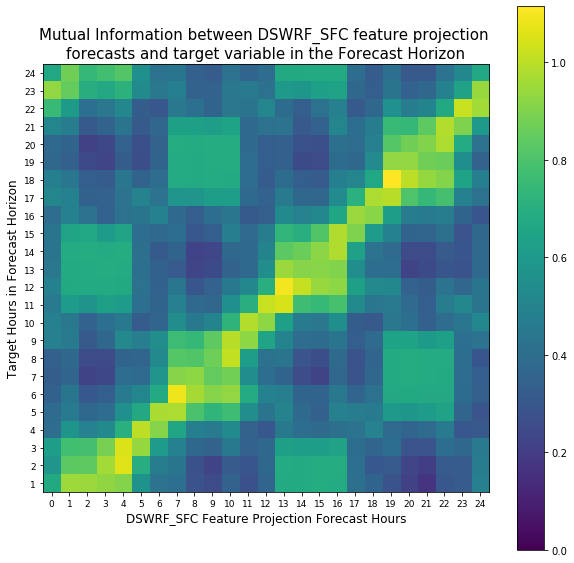
\includegraphics[width=0.65\textwidth]{chapter3/fig_mi_forecast_target.png}
    	\label{fig:fig_mi_forecast_target}
    	\caption[Mutual information between Downward Shortwave Radiation Flux feature projection forecasts and irradiance observations for target hours in the forecast horizon from Solar Array B]{Mutual information between feature projection forecasts of Downward Shortwave Radiation Flux (DSWRF\_SFC) and irradiance observations for target hours in the forecast horizon on Solar Array B.}
    \end{center}
\end{figure}

From among the weather parameters, downward shortwave radiation flux (DSWRF\_SFC), synonymous with global horizontal irradiance (GHI) has the maximum dependency on the target irradiance observations from all the three arrays. In \cite{Zach_Thesis}, all the 36 feature projections at a one-hour temporal resolution for each of the environmental attributes were used as the features for the machine learning models. However, as shown in Fig. \ref{fig:fig_mi_forecast_target}, it can be observed that the irradiance observations from solar array B for the target hours in the forecast horizon are dependent on only a certain number of feature projections in the forecast horizon. Thus, for each of the target hour, feature projections from 6 hours ahead, and 6 hours prior were used in a cyclic manner, which, owing to the 24 hour forecast horizon, would increase the chances of having similar weather conditions at the same hour the previous day or the following day.

Thus, the machine learning models used for postprocessing solar irradiance had 13 feature projections each for the four environmental attributes as described earlier, eight temporal features (four for the reference time of the observation, four for the target hour offset from the reference time), with irradiance observations from each of the solar arrays A, B and E as the response variables. 




\subchapter{Experiment Setup}


\subsubchapter{Multi-Model Blending Approach }
\par Describe pyranometers and corresponding PVLIB modeling technique contrast


\subsubchapter{Geographic Expansion of Forecast Coverage}

\begin{figure}[htbp]
    \begin{center}
    	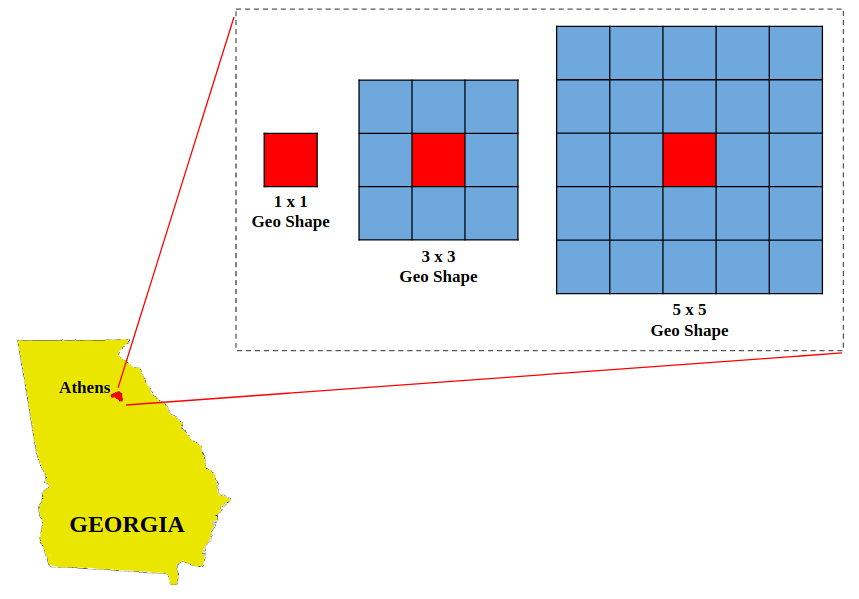
\includegraphics[width=0.65\textwidth]{chapter3/fig_geoshapes.png}
    	\label{fig:fig_geoshapes}
    	\caption[Geographic expansion of forecast coverage around Athens NAM model data grid]{Geographic expansion of forecast coverage with 1 x 1 Geo Shape representing Athens NAM model data grid, 3 x 3 Geo Shape and 5 x 5 Geo Shape representing grid of cells around Athens.}
    \end{center}
\end{figure}


\par Insert image with GA and corresponding grid extension



\subchapter{Results and Discussion}
Lorem ipsum dolor sit amet, consectetur adipiscing elit, sed do eiusmod tempor incididunt ut labore et dolore magna aliqua. Ut enim ad minim veniam, quis nostrud exercitation ullamco laboris nisi ut aliquip ex ea commodo consequat. Duis aute irure dolor in reprehenderit in voluptate velit esse cillum dolore eu fugiat nulla pariatur. Excepteur sint occaecat cupidatat non proident, sunt in culpa qui officia deserunt mollit anim id est laborum.

\begin{table}[h]
\begin{center}
    \caption{Sample Table 1}
    \begin{tabular}{ c c c c }
    	\toprule
    	col1 & col2 & col3 & col 4 \\
    	\midrule
    	\multirow{3}{4em}{Multiple row} & cell2 & cell3 & cell4\\ &
    	cell5 & cell6 & cell7 \\ &
    	cell8 & cell9 & cell10 \\
    	\midrule
    	\multirow{3}{4em}{Multiple row} & cell2 & cell3 & cell4 \\ &
    	cell5 & cell6 & cell7 \\ &
    	cell8 & cell9 & cell10 \\
    	\bottomrule
    \end{tabular}
\end{center}
\end{table}

Lorem ipsum dolor sit amet, consectetur adipiscing elit, sed do eiusmod tempor incididunt ut labore et dolore magna aliqua. Ut enim ad minim veniam, quis nostrud exercitation ullamco laboris nisi ut aliquip ex ea commodo consequat. Duis aute irure dolor in reprehenderit in voluptate velit esse cillum dolore eu fugiat nulla pariatur. Excepteur sint occaecat cupidatat non proident, sunt in culpa qui officia deserunt mollit anim id est laborum.

\newpage